\documentclass[aspectratio=149]{beamer}
% The values that it accepts are: 1610, 169, 149, 54, 43 and 32, which stand for the ratios 16:10, 16:9, 14:9, 5:4, 4:3 and 3:2, respectively.

% Idioma y codificacion en castellano
\usepackage[T1]{fontenc}
\usepackage[utf8]{inputenc}
\usepackage[english, spanish, es-tabla]{babel}

% Otros
\usepackage{fontspec}
\usepackage{unicode-math}
\usepackage{lmodern}
\usepackage{setspace}
\usepackage{csquotes}

% Imagenes
\usepackage{graphicx}
\graphicspath{{img/}}

% Bibliografía
\usepackage{biblatex}
\addbibresource{bibliografia.bib}

% Colores
\definecolor{link}{rgb}{0,0.4,0.6}
\definecolor{url}{rgb}{0.6,0,0}

% TODO list
\usepackage{pifont}
\usepackage{amssymb}

% Enlaces
\hypersetup{
    colorlinks = false,
    linktocpage = true,
    urlcolor = {url},
    linkcolor = {link},
    citecolor = {citation},
    pdfpagemode = {UseOutlines},
    pdfstartview = {Fit}}

% Titulo
\titlegraphic{
    \begin{center}
        
\includegraphics[height=2cm]{img/escudoUBU} \hspace{1cm}
        
\includegraphics[height=2cm]{img/escudoUVA} \hspace{1cm}
        
\includegraphics[height=2cm]{img/escudoULE} \vspace{1cm}
    \end{center}}

\setbeamertemplate{title page}{
    \begin{center}
        \vspace{0.4cm}
        {\textbf{\LARGE\inserttitle}}\\[0.8cm]
        \fontfamily{ptm}\selectfont
        {\insertauthor}\\[0.4cm]
        {\scriptsize\insertinstitute}\\[0.25cm]
        {\insertdate}\\[0.5cm]
        \inserttitlegraphic
    \end{center}}

%%% =========================
%%%  Nouveaux environnements
%%% =========================

%% Environnements pour les demo de code; tirés du document
%% principal. (L'environnement 'eqxample' ajoute des filets de part
%% et d'autre du bloc pour illustrer les marges.)
\newenvironment{demo}{%
    \begin{beamercolorbox}[wd=\linewidth,sep=6pt]{block body example}}
    {\end{beamercolorbox}}

\newenvironment{texample}[1][0.45\linewidth]{%
    \noindent\begin{minipage}{#1}%
    \def\producing{\end{minipage}\hfill\begin{minipage}{\dimexpr0.9\linewidth-#1}%
        \hbox\bgroup\kern-.2pt%
        \vbox\bgroup\parindent0pt\relax
        % The 3pt is to cancel the -\lineskip from \displ@y
        \abovedisplayskip3pt \abovedisplayshortskip\abovedisplayskip
        \belowdisplayskip0pt \belowdisplayshortskip\belowdisplayskip
        \noindent}
    }{%
        \par
        % Ensure that a lonely \[\] structure doesn't take up width less than
        % \hsize.
        \hrule height0pt width\hsize
        \egroup\kern-.2pt\egroup
        \end{minipage}%
        \par
    }

\newenvironment{eqxample}{%
    \noindent\begin{minipage}{.45\linewidth}%
    \def\producing{\end{minipage}\hfill\begin{minipage}{.45\linewidth}%
        \hbox\bgroup\kern-.2pt\vrule width.2pt%
        \vbox\bgroup\parindent0pt\relax
        % The 3pt is to cancel the -\lineskip from \displ@y
        \abovedisplayskip3pt \abovedisplayshortskip\abovedisplayskip
        \belowdisplayskip0pt \belowdisplayshortskip\belowdisplayskip
        \noindent}
    }{%
        \par
        % Ensure that a lonely \[\] structure doesn't take up width less than
        % \hsize.
        \hrule height0pt width\hsize
        \egroup\vrule width.2pt\kern-.2pt\egroup
        \end{minipage}%
        \par
  }

%% Simplfication de l'environnement 'quote' de beamer
\renewenvironment{quote}{%
    \begin{beamercolorbox}[wd=\linewidth,sep=6pt]{block body example}}
    {\end{beamercolorbox}}

%% Exercices
\newenvironment{exercice}{%
    \begin{frame}[fragile=singleslide]
    \frametitle{\faCogs\; Exercice}}{\end{frame}}
  
%%% =======
%%%  Varia
%%% =======

%% Longueurs pour la composition des pages couvertures avant et
%% arrière.
\newlength{\banderougewidth} \newlength{\banderougeheight}
\newlength{\bandeorwidth}    \newlength{\bandeorheight}
\newlength{\imageheight}
\newlength{\logoheight}

\mode<presentation> {
    \usetheme{ulaval}
    \setbeamercovered{transparent}
    \setbeamertemplate{navigation symbols}{}
}

\newenvironment{xframe}[2][]
    {\begin{frame}[fragile,environment=xframe,#1]
    \font
    \frametitle{#2}}
    {\end{frame}}

\AtBeginSection[]{
    \begin{frame}
    \huge \centerline{\insertsection}
    \small \tableofcontents[currentsection, hideothersubsections]
    \end{frame}
}

\setcounter{tocdepth}{2}
\newcommand{\acc}[1]{\textcolor{ulred}{\textbf{#1}}}


\title[Automatización del proceso de adquisición de imágenes de redes sociales para sistemas de recomendación]{Automatización del proceso de adquisición de imágenes de redes sociales para sistemas de recomendación}

\author[Daniel González Alonso]{
    Autor: Daniel González Alonso\\[1ex] 
    Tutor: Ángel Manuel Guerrero Higueras}

\institute[Universidad de Valladolid]{
    Máster Universitario en Inteligencia de Negocio \\[-4pt]
    y Big Data en Entornos Seguros}

\begin{document}

%==============================================================================
% Título
%==============================================================================
\begin{frame}[label=title, plain]
    \titlepage
\end{frame}

%==============================================================================
% TABLA DE CONTENIDOS
%==============================================================================
\begin{frame}[label=toc]{Tabla de contenidos}
 \setlength{\leftskip}{5cm}%
 \tableofcontents[subsectionstyle=hide]
\end{frame}

%==============================================================================
% INTRODUCCION
%==============================================================================
\section{Introducción}
\begin{frame}[label=intro]{Introducción}
    \begin{itemize}
        \item El turismo es una de las actividades económicas más importantes de España, pero con la pandemia de COVID-19 el sector turístico se vio gravemente afectado.
        \item Para recuperar los niveles de turismo previos es necesario potenciar el turismo, y uno de los posibles medios que se pueden aprovechar son las redes sociales.
        \item Instagram es muy popular en la actualidad, sobre todo para compartir lugares visitados y experiencias.
        \item Las publicaciones mostradas en cada búsqueda se basan en la cadena de búsqueda, cuentas seguidas y popularidad. Una posible mejora es basarse en las características de la persona que hace la búsqueda.
    \end{itemize}
\end{frame}

%==============================================================================
% OBJETIVOS
%==============================================================================
\section{Objetivos}
\begin{frame}[label=objetivos]{Objetivos}
    \begin{itemize}
        \item \textbf{Objetivos generales}: conocer el estado del arte, desarrollar el software necesario para descargar y analizar las publicaciones, y hacer una visualización de los datos.
        \item \textbf{Objetivos técnicos}: uso de herramientas en la nube para el alojamiento y procesamiento de datos, el proyecto no ha de suponer ningún coste, y se busca crear un cuadro de mandos para la visualización.
        \item \textbf{Objetivos personales}: aprender a usar herramientas y servicios en la nube, mejorar mis conocimientos sobre almacenamiento y procesado de grandes cantidades de datos, y poner en práctica mis conocimientos sobre cuadros de mando.
    \end{itemize}
\end{frame}

%==============================================================================
% TRABAJOS RELACIONADOS
%==============================================================================
\section{Trabajos Relacionados}
\begin{frame}[label=relat]{Trabajos Relacionados}
    \begin{itemize}
        \item Recomendación de contenido:
        \begin{itemize}
            \item Rastogi et al. \cite{sent_analysis_facebook_user_recom} emplea análisis de sentimiento en publicaciones de Facebook para mejorar los resultados de las recomendaciones de usuarios.
            \item Khan et al. \cite{pers_tweet_recomendation} propone un sistema de recomendación de tweets dentro del dominio de la salud.
        \end{itemize}
        \item Recomendación de lugares:
        \begin{itemize}
            \item Xi Shao et al. \cite{8796367} presenta un sistema de recomendación de turismo personalizado denominado SMTM.
            \item Shafqat et al. \cite{recom_mech_under_emph} propone un sistema de recomendación de turismo teniendo en cuenta lugares poco enfatizados.
        \end{itemize}
        \item Análisis sobre destinos turísticos:
        \begin{itemize}
            \item Paolanti et al. \cite {tourism_dest_rec_geolocation} comparan el rendimiento de múltiples métodos actuales de aprendizaje profundo sobre tweets relacionados con Cilento, Italia.
            \item Borrajo-Millán et al. \cite{su13116015} llevan a cabo un análisis sobre el turismo en España y la percepción que tienen los turistas chinos.
        \end{itemize}
    \end{itemize}
\end{frame}

%==============================================================================
% TECNICAS Y HERRAMIENTAS
%==============================================================================
\section{Técnicas y Herramientas}
\begin{frame}[label=herramientas]{Técnicas y Herramientas}
    \begin{itemize}
        \item \textbf{Instalooter}
        \item Servicios en la nube con \textbf{Amazon Web Services}:
        \begin{itemize}
            \item Rekognition
            \item Amazon S3
            \item Amazon EC2
            \item DynamoDB
            \item AWS Lambda
            \item Amazon API Gateway
        \end{itemize}
        \item \textbf{Grafana}
        \item Otras herramientas:
        \begin{itemize}
            \item \texttt{virtualenv}
            \item Visual Studio Code
            \item Git y GitHub
            \item \LaTeX y Overleaf
        \end{itemize}
    \end{itemize}
\end{frame}

%==============================================================================
% ASPECTOS RELEVANTES DEL DESARROLLO DEL PROYECTO
%==============================================================================
\section{Aspectos relevantes del desarrollo del proyecto}

\subsection{Estudio preliminar}
\begin{frame}[label=preliminar]{Estudio preliminar}
    \begin{itemize}
        \item Se valoraron los distintos crawlers a utilizar para descargar publicaciones de instagram. Finalmente se seleccionó Instalooter.
        \item Se hicieron pruebas con Google Cloud y Cloud Vision. Tras ver que no se podía recuperar ni la edad ni el genero se decidió valorar otras posibilidades, como MS Azure y AWS.
        \item Se decidió usar AWS porque Rekognition permitía recuperar la información necesaria y porque con Azure no se podían crear máquinas virtuales por problemas de disponibilidad.
    \end{itemize}
\end{frame}

\subsection{Diseño e implementación de la base de datos}
\begin{frame}[label=bbdd]{Diseño e implementación de la base de datos}
    \begin{itemize}
        \item Se creó un script que descargaba las publicaciones (imagen y metadatos) en Amazon S3, las procesa con Rekognition, y guarda el resultado final en una base de datos de DynamoDB.
        \item La base de datos cuenta con una única tabla, cada entrada se corresponde con una cara e incluye tanto metadatos de Instalooter como la información obtenida con Rekognition.
    \end{itemize}

{\scriptsize
\begin{table}[H]
    \vspace{-0.4cm}
    \centering
    \begin{tabular}{|p{0.25\textwidth}|p{0.1\textwidth}|p{0.55\textwidth}|}
    \hline
	Nombre del campo & Tipo & Orígen \\ \hline
	id & Cadena & Instalooter.id \\ \hline
	faceIndex & Número & Índice de la cara en Rekognition.FaceDetails \\ \hline
	dTime & Cadena & Instalooter.taken\_at\_timestamp, formateado como \texttt{YYYY-MM-DDTHH:MM:SS} \\ \hline
	shortCode & Cadena & Instalooter.shortcode \\ \hline
	... & & \\ \hline
	confidence & Número & Rekognition.FaceDetails{[}*{]}.Confidence \\ \hline
	ageLow & Número & Rekognition.FaceDetails{[}*{]}.AgeRange.Low \\ \hline
	ageHigh & Número & Rekognition.FaceDetails{[}*{]}.AgeRange.High \\ \hline
	gender & Cadena & Rekognition.FaceDetails{[}*{]}.Gender.Value \\ \hline
	... & & \\ \hline
    \end{tabular}
    %\caption{Diseño de la tabla \texttt{valltourisminsta}}
    \label{tab:dynamodb_table}
\end{table}
}



\end{frame}

\subsection{Proceso de descarga de las publicaciones}
\begin{frame}[label=descarga]{Proceso de descarga de las publicaciones}
    \begin{itemize}
        \item Para llevar a cabo el proceso de descarga de publicaciones se tuvo que ejecutar el script de la sección anterior en varias ocasiones desde una máquina virtual de EC2.
        \item Para la descarga se emplea una la lista con 44 hashtags seleccionados manualmente.
        \item Se descargaron un total de 3916 publicaciones de Instagram debido al límite de subida de Amazon S3. Mediante Rekognition se extrajeron unas 5408 caras.
        \item En esta fase hubo que hacer una corrección a Instalooter porque dejó de funcionar.
    \end{itemize}
\end{frame}

\subsection{Visualización}
\begin{frame}[label=visualizacion1]{Visualización}
    \begin{itemize}
        \item Para llevar a cabo la visualización se valoraron varias herramientas:
        \begin{itemize}
            \item Web estática con ChartJS o D3JS: problema requiere mucho tiempo.
            \item QLik, MS PowerBI, Tableau: problema no tienen conectores gratuitos con DynamoDB y tienen un periodo de prueba limitado.
            \item Grafana: es open source pero tampoco tiene conector con DynamoDB.
        \end{itemize}
        \item Finalmente se decidió por Grafana que aunque no tiene conector, existen plugins que pueden ayudar a la implementación de un conector sencillo mediante APIs REST.
        \begin{figure}
            \centering
            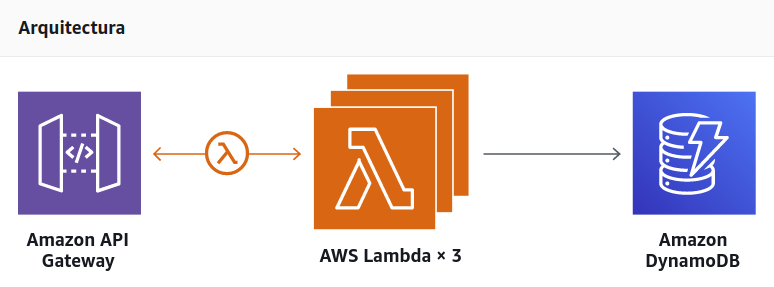
\includegraphics[width=0.75\textwidth]{img/gateway_flow.png}
            \label{fig:gate_flow}
        \end{figure}
    \end{itemize}
\end{frame}
\begin{frame}[label=visualizacion2]{Visualización}
    \begin{figure}
        \centering
        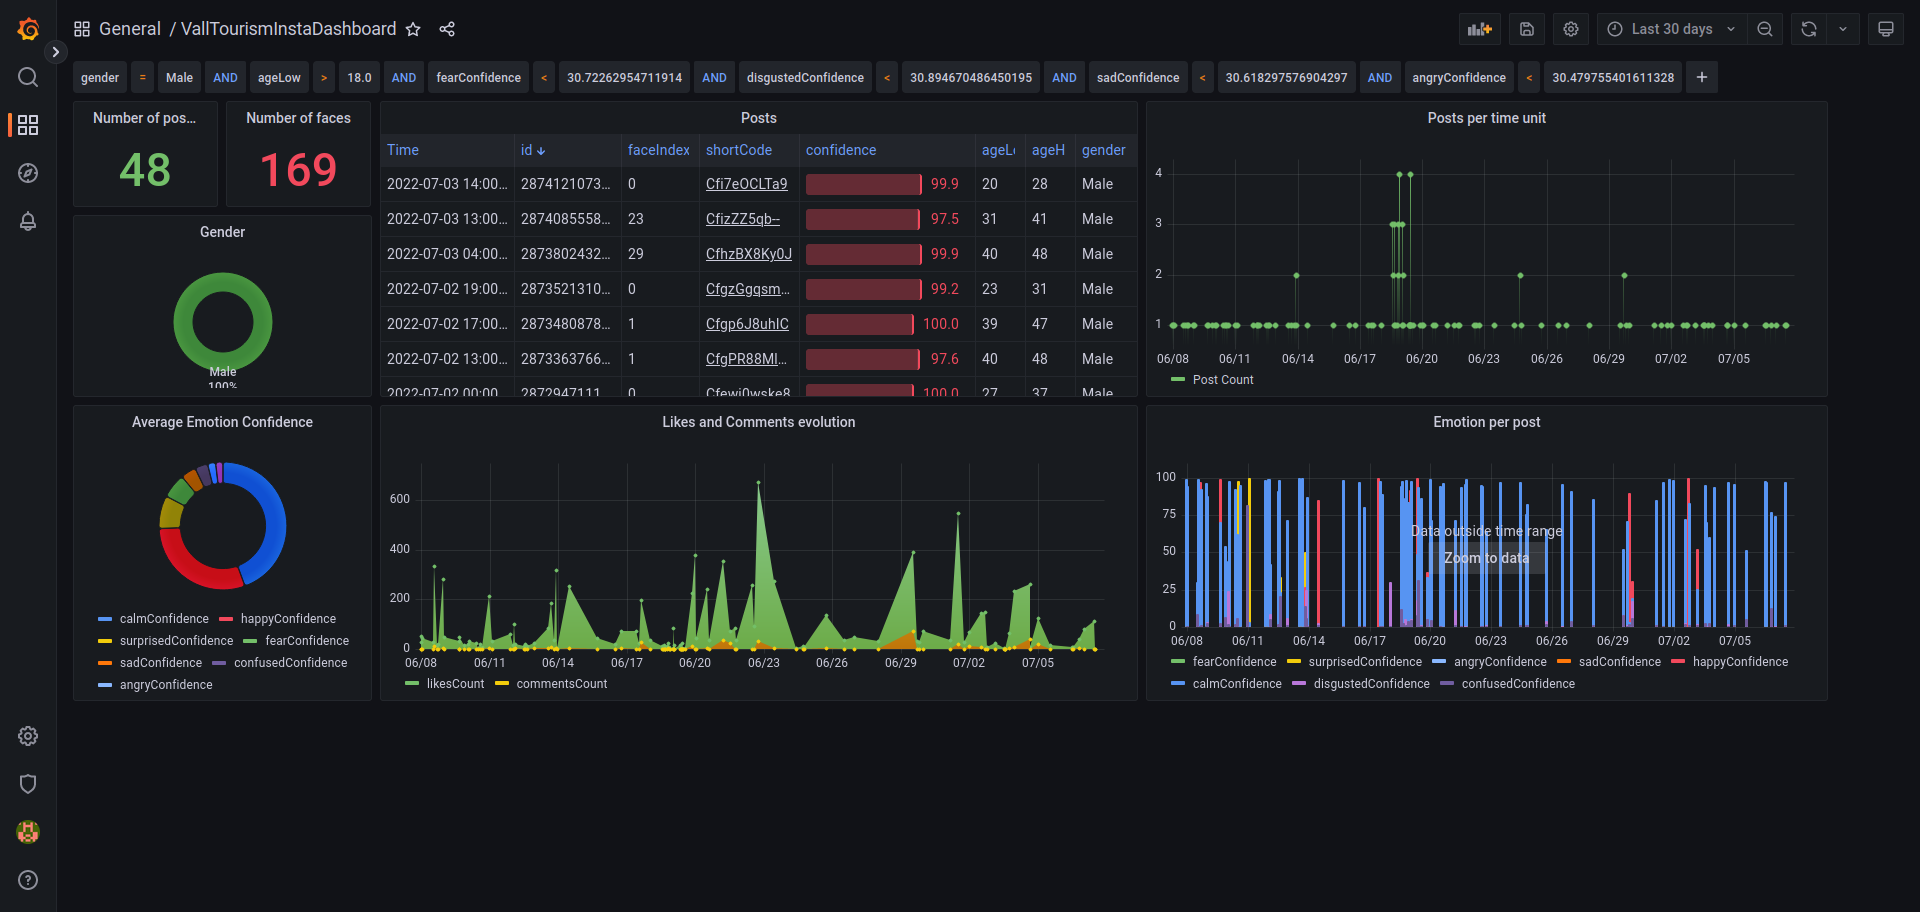
\includegraphics[width=1.0\textwidth]{img/dashboard.png}
        \label{fig:grafana}
    \end{figure}
\end{frame}

%==============================================================================
% CONCLUSIONES Y LINEAS DE TRABAJO FUTURAS
%==============================================================================
\section{Conclusiones y Líneas de trabajo futuras}

\subsection{Conclusiones}
\begin{frame}[label=conclu]{Conclusiones}
    \begin{itemize}
        \item Se considera que se ha conseguido cumplir los objetivos generales inicialmente planteados.
        \item La base base de datos final ha estado más limitada de lo esperado.
        \item Los crawlers son muy sensibles a las actualizaciones de las páginas web.
        \item Usar DynamoDB presenta algunas limitaciones, tanto por las consultas que se pueden hacer como por el soporte de otras herramientas para conectarse a esta base de datos.
    \end{itemize}
\end{frame}

\subsection{Líneas de trabajo futuras}
\begin{frame}[label=lineas]{Líneas de trabajo futuras}
    \begin{itemize}
        \item Agrandar la base de datos.
        \item Ejecutar descarga de datos periódicamente de forma automática, ya sea mediante un cron o en AWS Lambda.
        \item Explotar el texto de la descripción de las publicaciones.
        \item Desarrollar una aplicación o una página web que sea más \textit{user friendly} en vez de usar un cuadro de mandos.
    \end{itemize}
\end{frame}

%==============================================================================
% Bibliografía
%==============================================================================
\begin{frame}[allowframebreaks]{Referencias}
    \printbibliography
\end{frame}

\end{document}